\chapter{偏好与无差异曲线}
\label{chp:preferences-and-indifferent-curves}

假设给定两个消费束$A: (x_1,y_1)$与$B: (x_2,y_2)$,消费者可按照他自己的意愿对这两个消费束排序。即消费者可以认为一个消费束严格好于另外一个消费束,或者认为这两个消费束无差异。

我们用符号$\succ$表示\emph{严格偏好}\index{preference 偏好!strict 严格偏好},因此$A \succ B$表示消费者严格偏好$(x_1,y_1)$胜于$(x_2,y_2)$,意思是说他肯定想要消费束$A$而不是消费束$B$。这种偏好关系提供了判断消费者选择哪个消费束的依据。如果消费者偏好消费束$A$胜于消费束$B$,那么他会选择消费束$A$。因此,偏好的思想是基于消费者行为之上的。

\emph{无差异的}\index{preference 偏好!indifferent (偏好是)无差异的},用符号$\sim$表示。$(x_1,y_1) \sim (x_2,y_2)$表示消费者根据自己的偏好,认为这两个消费束$A$和$B$提供的满足程度是一样的。

\emph{弱偏好}\index{preference 偏好! weak 弱偏好},用符号$\succeq$表示。$(x_1,y_1) \succeq (x_2,y_2)$指的是消费者对于前者的偏好胜于后者或者对于这两个消费束无差异,即消费者认为前者至少与后者一样好。

\section{偏好的公理性假设}
消费者理论的公理性假设:
\begin{compactitem}
\item \emph{完备性公理}:假设任何两个消费束都可以比较,即给定消费束$A$和消费束 $B$,必有$(x_1,y_1) \succeq (x_2,y_2)$;或者$(x_2,y_2) \succeq (x_1,y_1)$;或者二者都成立,即消费者对于这两个消费束是无差异的。
\item \emph{反身性公理}:假设任何消费束都至少和它本身一样好,即$(x_1,y_1) \succeq (x_1,y_1)$。
\item \emph{传递性公理}:如果$(x_1,y_1) \succeq (x_2,y_2)$,并且$(x_2,y_2) \succeq (x_3,y_3)$,则$(x_1,y_1) \succeq (x_3,y_3)$。即,如果消费者认为消费束$A$至少和$B$一样好,而且$B$至少与$C$一样好,则他认为消费束$A$与$C$至少一样好。
\end{compactitem}

\section{良性偏好}
\index{preference 偏好!well-behaved 良性偏好}
\label{sec:well-behaved-preference}

第一个假设:\emph{局部餍足性}又称\emph{局部非饱和性},指的是任何消费都不存在充分满足。其意义是指不存在任何消费束令消费者达到满足的极限,总有更偏好的消费束存在。对于任意的$(x_1,y_1)$,总可以找到另一个消费束$x_2,y_2$使得$(x_2, y_2) \succ (x_1, y_1)$。

第一个假设:连续性,无差异集合的图形是一个连续的曲面。

草稿:第一个假设:在没有达到饱和点之前\emph{偏好具有单调性},或者说\emph{多多益善}。

给定两个消费束$(x_1, y_1)$和$(x_2, y_2)$,如果$x_2 \geq x_1$且$y_2 > y_1$或者$x_2 > x_1$且$y_2 \geq y_1$,则必有$(x_2, y_2) \succ (x_1, y_1)$。这表示我们研究的商品对象为 goods(好的、想要的商品),而非 bads(坏的、厌恶的商品)。

从几何上偏好的单调性假设决定了无差异曲线的斜率是负的。对于一个给定的消费束$(x_1, y_1)$,如果增大$x1$的消费数量至$(x_1 + a, y_1)$,则$(x_1 + a, y_1) \succ (x_1, y_1)$。这时只有减少$y$的消费数量至$(x_1 + a, y_1 -b)$才有可能使得$(x_1 + a, y_1 -b) \sim (x_1, y_1)$。

第二个假设:凸性,\emph{平均束好于端点束},即在一条无差异曲线上任取两个消费束,二者连线上的任意一个消费束(端点除外)都弱偏好或者严格偏好于端点消费束。

\begin{figure}[!h]
\colorbox{black!3}{\parbox{\linewidth-2\fboxsep}{%
\centering
\begin{subfigure}[b]{0.5\textwidth}
\centering
%%%%%%%%%%%%%%%%%%%%%%%%%%%%%%
\begin{tikzpicture}
\begin{axis}[
	axis background/.style={fill=blueL},
	domain=0:9,
	xmin=0,xmax=6,ymin=0,ymax=6,
	xlabel style={below},xlabel=$X$,
	ylabel style={left},ylabel=$Y$,
	enlargelimits=false,samples=300]
\addplot[fill=white,draw=none]
	{4/x} \closedcycle;
\addplot[ultra thick,draw=blue]
	{4/x};
\addplot[only marks,forget plot,black,mark options={mark size=1.25pt,fill=white},mark=*]
	coordinates {(1,4) (2,3) (4,1)};
\addplot[white,dashed]
	coordinates {(1,4) (4,1)};
\draw (axis cs:1,4) node[left] {$A$};
\draw (axis cs:2,3) node[right] {$M$};
\draw (axis cs:4,1) node[below] {$B$};
\end{axis}
\end{tikzpicture}
\caption{凸性偏好}
\label{fig:convex-preferences}
\end{subfigure}%
\begin{subfigure}[b]{0.5\textwidth}
\centering
%%%%%%%%%%%%%%%%%%%%%%%%%%%%%%
\begin{tikzpicture}
\begin{axis}[
	axis background/.style={fill=blueL},
	domain=0:9,
	xmin=0,xmax=6,ymin=0,ymax=6,
	xlabel style={below},xlabel=$X$,
	ylabel style={left},ylabel=$Y$,
	enlargelimits=false,samples=300]
\addplot[domain=0:4.2,fill=white,draw=none]
	{5-4/(5-x)} \closedcycle;
\addplot[ultra thick,domain=0:4.2,blue]
	{5-4/(5-x)};
\addplot[only marks,forget plot,black,mark options={mark size=1.25pt,fill=white},mark=*]
	coordinates {(1,4) (3,2) (4,1)};
\addplot[gray,dashed]
	coordinates {(1,4) (4,1)};
\draw (axis cs:1,4) node[below] {$A$};
\draw (axis cs:3,2) node[left] {$M$};
\draw (axis cs:4,1) node[left] {$B$};
\end{axis}
\end{tikzpicture}
\caption{凹性偏好}
\label{fig:concave-preferences}
\end{subfigure}
\caption{偏好类型举例}
\label{fig:convex-and-concave-preferences}%
}}
\end{figure}

\section{无差异曲线的意义}

\begin{figure}[!h]
\colorbox{black!3}{\parbox{\linewidth-2\fboxsep}{%
\centering
\begin{subfigure}[b]{0.5\textwidth}
\centering
%%%%%%%%%%%%%%%%%%%%%%%%%%%%%%
\begin{tikzpicture}
\begin{axis}[
	axis background/.style={fill=blueL},
	domain=0:9,
	extra x ticks={1,2.5,4},
	extra x tick style={tickwidth=0},
	extra x tick labels={{$x_1$},{$x_w$},{$x_2$}},
	extra y ticks={1,2.5,4},
	extra y tick style={tickwidth=0},
	extra y tick labels={{$y_2$},{$y_w$},{$y_1$}},
	xmin=0,xmax=6,ymin=0,ymax=6,
	xlabel style={below},xlabel=$X$,
	ylabel style={left},ylabel=$Y$,
	enlargelimits=false,samples=300]
\addplot[fill=white,draw=none]
	{4/x} \closedcycle;
\addplot[ultra thick,draw=blue]
	{4/x};
\addplot[only marks,forget plot,black,mark options={mark size=1.25pt,fill=white},mark=*]
	coordinates {(1,4) (2.5,2.5) (4,1)};
\addplot[white,dashed]
	coordinates {(1,4) (4,1)};
\addplot[gray,very thin,dashed] coordinates {(0,4) (1,4) (1,0)};
\addplot[gray,very thin,dashed] coordinates {(0,1) (4,1) (4,0)};
\addplot[gray,very thin,dashed] coordinates {(0,2.5) (2.5,2.5) (2.5,0)};
\draw (axis cs:1,4) node[left] {$A$};
\draw (axis cs:2.5,2.5) node[above right] {$W$};
\draw (axis cs:4,1) node[above right] {$B: B \sim A$};
\draw (axis cs:4,4) node {弱偏好集:$W \succeq A$};
\end{axis}
\end{tikzpicture}
\caption{无差异曲线与弱偏好集}
\label{fig:indifferent-curve-and-weak-preferences}
\end{subfigure}%
\begin{subfigure}[b]{0.5\textwidth}
\centering
%%%%%%%%%%%%%%%%%%%%%%%%%%%%%%
\begin{tikzpicture}
\begin{axis}[
	domain=0:10,
	xmin=0,xmax=9.5,ymin=0,ymax=9.5,
	xlabel style={below},xlabel=$X$,
	ylabel style={left},ylabel=$Y$,
	enlargelimits=false,samples=300]
\addplot graphics[xmin=0,xmax=9.5,ymin=0,ymax=9.5] {densityplot};
\addplot[cm={0,1,1,0,(0,0)},draw=white,domain=2.36:9.5] {125/(x^3)};
\addplot[cm={0,1,1,0,(0,0)},draw=white,domain=4.91:9.5] {1125/(x^3)};
\addplot[cm={0,1,1,0,(0,0)},draw=white,domain=6.07:9.5] {2125/(x^3)};
\addplot[cm={0,1,1,0,(0,0)},draw=white,domain=6.90:9.5] {3125/(x^3)};
\addplot[cm={0,1,1,0,(0,0)},draw=white,domain=7.57:9.5] {4125/(x^3)};
\end{axis}
\end{tikzpicture}
\caption{无差异曲线(等高线图与密度图)}
\label{fig:midudenggao-of-indifferent-curves}%
\end{subfigure}%
\caption{无差异曲线的意义}
\label{fig:meaning-of-indifferent-curves}%
}}
\end{figure}

\begin{Definition}[无差异曲线]\index{indifferent curves 无差异曲线}
无差异曲线是用来表示消费者偏好相同的两种商品的所有组合的。或者说,它是表示能够给消费者带来相同的效用水平或满足程度的两种商品的所有组合的。\cite{courant2001chs}
\end{Definition}

绘制示意图的时候往往选择“疏密适中”的三四条“等高线”作为代表,我们所关注的只是无差异曲线的个体形态和整体次序,他们的疏密是无意义的——这和带有基数特征的等产量线是不同的(第\pageref{subsec:returns-to-scale-of-linear-production-function}页\ref{subsec:returns-to-scale-of-linear-production-function}小节)。对效用函数的单调变换不会影响序数论的效用分析,反面来看就是说效用分析中不存在“规模报酬”。例如$u=x y^3$和$u=x^{1/4} y^{3/4}$所描述的偏好是一致的。


由于假设效用函数的连续性,如果用色彩深浅代表效用水平的高低,那么整个无差异曲线系统使用密度图或者三维空间的曲面表示更直观一些。限于我的编辑能力和所选软件的限制仅能退而求其次了。

\begin{figure}[!h]
\begin{shaded*}
\begin{minipage}[t]{0.5\linewidth} 
\centering 
%\vspace{0pt}
\begin{tikzpicture}
%(x^0.5 + 1) (y^0.5 + 1) - 1
\begin{axis}[
domain=0:10,
axis on top=true,
view={-45}{45},%view={-25}{60},
xmin=0,xmax=10,ymin=0,ymax=10,zmin=0,zmax=18,
xtick=\empty,ytick=\empty,ztick=\empty,
xticklabel=\ ,yticklabel=\ ,zticklabel=\ ,
width=180pt,height=150pt,
scale only axis,
axis x line*=middle,
axis y line*=middle,
axis z line*=none,
axis line style={-},
extra x ticks={9},
extra x tick style={tickwidth=0},
extra x tick labels={$x$},
extra y ticks={9},
extra y tick style={tickwidth=0},
extra y tick labels={$y$},
extra description/.code={
	\node[below] at (axis cs:0,0,0) {$O$};
	\node[above] at (axis cs:10,10,17) {$z$};
},
axis background/.style={fill=black!3}]
\addplot3[fill=white,draw=none] coordinates {
(0,0,0)
(0,10,0)
(10,10,0)
(10,0,0)
};
%\addplot3 table[x=x,y=y,z=z] {pgfplots_scatterdata4.dat};

%\addplot3[left color=green,right color=green,middle color=yellow,draw=none]
\addplot3[fill=green,fill opacity=0.5,draw=none]
coordinates {
(2.29814,10.00001158,9.472)
(2.3,9.993596697,9.472)
(2.45,9.500635151,9.472)
(2.6,9.051357661,9.472)
(2.75,8.640028364,9.472)
(2.9,8.261899936,9.472)
(3.05,7.913005333,9.472)
(3.2,7.590000799,9.472)
(3.35,7.290045837,9.472)
(3.5,7.01071027,9.472)
(3.65,6.74990144,9.472)
(3.8,6.505806579,9.472)
(3.95,6.276846753,9.472)
(4.1,6.061639726,9.472)
(4.25,5.85896977,9.472)
(4.4,5.667762939,9.472)
(4.55,5.487066676,9.472)
(4.7,5.316032881,9.472)
(4.85,5.153903771,9.472)
(5,5,9.472)
(5.15,4.85371063,9.472)
(5.3,4.714484617,9.472)
(5.45,4.581823552,9.472)
(5.6,4.455275445,9.472)
(5.75,4.334429378,9.472)
(5.9,4.218910884,9.472)
(6.05,4.108377952,9.472)
(6.2,4.002517541,9.472)
(6.35,3.901042542,9.472)
(6.5,3.803689123,9.472)
(6.65,3.710214386,9.472)
(6.8,3.620394317,9.472)
(6.95,3.534021962,9.472)
(7.1,3.45090582,9.472)
(7.25,3.370868413,9.472)
(7.4,3.293745016,9.472)
(7.55,3.219382518,9.472)
(7.7,3.14763841,9.472)
(7.85,3.078379876,9.472)
(8,3.011482974,9.472)
(8.15,2.9468319,9.472)
(8.3,2.884318331,9.472)
(8.45,2.823840821,9.472)
(8.6,2.765304262,9.472)
(8.75,2.708619394,9.472)
(8.9,2.653702357,9.472)
(9.05,2.600474289,9.472)
(9.2,2.548860954,9.472)
(9.35,2.498792408,9.472)
(9.5,2.450202691,9.472)
(9.65,2.403029543,9.472)
(9.8,2.357214152,9.472)
(9.95,2.312700911,9.472)
(10,2.298143356,9.472)
(10,2.298143356,0)
(9.95,2.312700911,0)
(9.8,2.357214152,0)
(9.65,2.403029543,0)
(9.5,2.450202691,0)
(9.35,2.498792408,0)
(9.2,2.548860954,0)
(9.05,2.600474289,0)
(8.9,2.653702357,0)
(8.75,2.708619394,0)
(8.6,2.765304262,0)
(8.45,2.823840821,0)
(8.3,2.884318331,0)
(8.15,2.9468319,0)
(8,3.011482974,0)
(7.85,3.078379876,0)
(7.7,3.14763841,0)
(7.55,3.219382518,0)
(7.4,3.293745016,0)
(7.25,3.370868413,0)
(7.1,3.45090582,0)
(6.95,3.534021962,0)
(6.8,3.620394317,0)
(6.65,3.710214386,0)
(6.5,3.803689123,0)
(6.35,3.901042542,0)
(6.2,4.002517541,0)
(6.05,4.108377952,0)
(5.9,4.218910884,0)
(5.75,4.334429378,0)
(5.6,4.455275445,0)
(5.45,4.581823552,0)
(5.3,4.714484617,0)
(5.15,4.85371063,0)
(5,5,0)
(4.85,5.153903771,0)
(4.7,5.316032881,0)
(4.55,5.487066676,0)
(4.4,5.667762939,0)
(4.25,5.85896977,0)
(4.1,6.061639726,0)
(3.95,6.276846753,0)
(3.8,6.505806579,0)
(3.65,6.74990144,0)
(3.5,7.01071027,0)
(3.35,7.290045837,0)
(3.2,7.590000799,0)
(3.05,7.913005333,0)
(2.9,8.261899936,0)
(2.75,8.640028364,0)
(2.6,9.051357661,0)
(2.45,9.500635151,0)
(2.3,9.993596697,0)
(2.29814,10.00001158,0)
};

%----------------------------------------------------------------------
%补偿z轴
%\addplot3[black] coordinates {
%(10,10,16.325)
%(10,10,18)
%};
%补偿坐标系边框
\addplot3[gray,dashed,thin] coordinates {
(0,10,0)
(10,10,0)
(10,0,0)
};
%补偿z轴
\addplot3[gray,dashed,thin] coordinates {
(10,10,0)
(10,10,16.324)
};
%补偿xymax的纵向边界
\addplot3[gray,dashed,thin] coordinates {
(0,10,0)
(0,10,3.163)
};
\addplot3[gray,dashed,thin] coordinates {
(10,0,0)
(10,0,3.163)
};

\addplot3 graphics[
points={%important
(10,0,3.16) => (600,180)
(8,8,8) => (301,318)
(10,10,16.325) => (301,464)
(0,0,0) => (301,1)
}] {qumianq.png};

%----------------------------------------------------------------------
%z=z(2.5,2.5)=5.66228 的无差异曲线
%x=0.36076, y=10
%x=10, y=0.36076
\addplot3[draw=green,ultra thick,domain=0.36076:10,samples=40,samples y=0] ({x},{((2.5^0.5+1)^2/(x^0.5 + 1) - 1)^2},{5.66228}); 
\addplot3[draw=gray,domain=0.36076:10,samples=40,samples y=0,dashed] ({x},{((2.5^0.5+1)^2/(x^0.5 + 1) - 1)^2},{0}); 
\addplot3[gray,dashed,thin] coordinates {
(10,0.36076,0)
(10,0.36076,5.66228)
};
\addplot3[gray,dashed,thin] coordinates {
(0.36076,10,0)
(0.36076,10,5.66228)
};
\node[above] at (axis cs:0.36076,10,5.66228) {$A$};
\node[above] at (axis cs:10,0.36076,5.66228) {$B$};

%----------------------------------------------------------------------
%z=z(5,5)=9.472 的无差异曲线
%x=2.29814, y=10
%x=10, y=2.29814
\addplot3[draw=green,ultra thick,domain=2.29814:10,samples=40,samples y=0] ({x},{((5^0.5+1)^2/(x^0.5 + 1) - 1)^2},{9.472}); 
\addplot3[draw=gray,domain=2.29814:10,samples=40,samples y=0,dashed] ({x},{((5^0.5+1)^2/(x^0.5 + 1) - 1)^2},{0}); 
\addplot3[gray,dashed,thin] coordinates {
(10,2.29814,0)
(10,2.29814,9.472)
};
\addplot3[gray,dashed,thin] coordinates {
(2.29814,10,0)
(2.29814,10,9.472)
};
\node[above] at (axis cs:2.29814,10,9.472) {$C$};
\node[above] at (axis cs:10,2.29814,9.472) {$D$};
\node[below] at (axis cs:2.29814,10,0) {$C'$};
\node[below] at (axis cs:10,2.29814,0) {$D'$};
%----------------------------------------------------------------------
% z = z(7.5,7.5) = 12.9772 的无差异曲线
% x = 5.5605, y = 10
% x = 10, y = 5.5605
\addplot3[draw=green,ultra thick,domain=5.5605:10,samples=40,samples y=0] ({x},{((7.5^0.5+1)^2/(x^0.5 + 1) - 1)^2},{12.9772}); 
\addplot3[draw=gray,domain=5.5605:10,samples=40,samples y=0,dashed] ({x},{((7.5^0.5+1)^2/(x^0.5 + 1) - 1)^2},{0}); 
\addplot3[gray,dashed,thin] coordinates {
(10,5.5605,0)
(10,5.5605,12.9772)
};
\addplot3[gray,dashed,thin] coordinates {
(5.5605,10,0)
(5.5605,10,12.9772)
};
\node[above] at (axis cs:5.5605,10,12.9772) {$E$};
\node[above] at (axis cs:10,5.5605,12.9772) {$F$};

%----------------------------------------------------------------------
%灰色的边界截面
%\addplot3[draw=none,fill=gray,fill opacity=0.75,samples=40,samples y=0] ({x},{0},{sqrt(x)}) \closedcycle;
\addplot3[draw=none,fill=gray,fill opacity=0.75,samples=40,samples y=0] ({x},{0},{sqrt(x)}) --cycle;
\addplot3[fill=gray,fill opacity=0.75,draw=none] coordinates {
(0,0,0)
(10,0,0)
(10,0,3.163)
};

\addplot3[draw=none,fill=gray,fill opacity=0.75,samples=40] ({0},{y},{sqrt(y)}) --cycle;
\addplot3[fill=gray,fill opacity=0.75,draw=none] coordinates {
(0,0,0)
(0,10,0)
(0,10,3.163)
};

%----------------------------------------------------------------------
%绘制曲面与坐标系边界的交线
%(x^0.5 + 1) (y^0.5 + 1) - 1
\addplot3[draw=red,thick,samples=40,samples y=0] ({x},{0},{sqrt(x)}); %samples=100,samples y=0
\addplot3[draw=red,thick,samples=60,samples y=0] ({x},{10},{4.16*(sqrt(x)+1)-1});
\addplot3[draw=blue,thick,samples=40] ({0},{y},{sqrt(y)});
\addplot3[draw=blue,thick,samples=40] ({10},{y},{4.16*(sqrt(y)+1)-1});
\end{axis}
\end{tikzpicture}
\caption{效用曲面与无差异曲线}
\label{fig:3d-indifferent-curves-a}
\end{minipage}% 
\begin{minipage}[t]{0.5\linewidth} 
\centering
%\vspace{0pt}
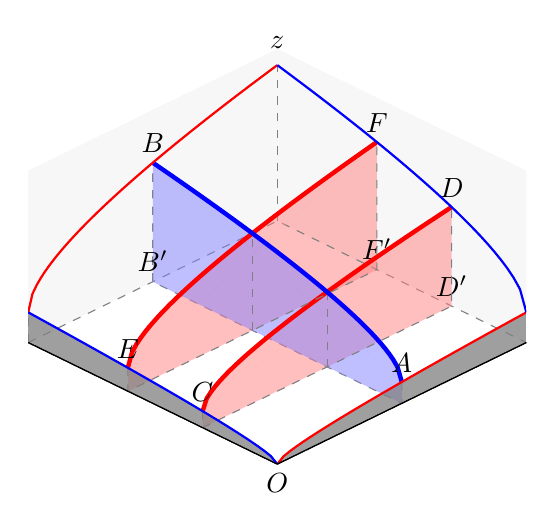
\begin{tikzpicture}
%(x^0.5 + 1) (y^0.5 + 1) - 1
\begin{axis}[
domain=0:10,
axis on top=true,
view={-45}{45},%view={-25}{60},
xmin=0,xmax=10,ymin=0,ymax=10,zmin=0,zmax=18,
xtick=\empty,ytick=\empty,ztick=\empty,
xticklabel=\ ,yticklabel=\ ,zticklabel=\ ,
width=180pt,height=150pt,
scale only axis,
axis x line*=middle,
axis y line*=middle,
axis z line*=none,
axis line style={-},
extra x ticks={5,9},
extra x tick style={tickwidth=0},
extra x tick labels={$A'$,$x$},
extra y ticks={3,6,9},
extra y tick style={tickwidth=0},
extra y tick labels={$C'$,$E'$,$y$},
extra description/.code={
	\node[below] at (axis cs:0,0,0) {$O$};
	\node[above] at (axis cs:10,10,17) {$z$};
},
axis background/.style={fill=black!3}]
\addplot3[fill=white,draw=none] coordinates {
(0,0,0)
(0,10,0)
(10,10,0)
(10,0,0)
};

\addplot3[gray,dashed,thin] coordinates {
(5,0,2.236)
(5,0,0)
(5,10,0)
(5,10,12.469)
};

\addplot3[fill=red!50,draw=none,fill opacity=0.5] coordinates {
(0,6,0)
(0,6,2.449)
(10,6,13.358)
(10,6,0)
};

%----------------------------------------------------------------------
\addplot3[gray,dashed,thin] coordinates {
(0,10,0)
(10,10,0)
(10,0,0)
};
%补偿z轴
\addplot3[gray,dashed,thin] coordinates {
(10,10,0)
(10,10,16.324)
};
%补偿xymax的纵向边界
\addplot3[gray,dashed,thin] coordinates {
(0,10,0)
(0,10,3.163)
};
\addplot3[gray,dashed,thin] coordinates {
(10,0,0)
(10,0,3.163)
};
%----------------------------------------------------------------------
%y=3 z=z(x) 观察x的边际效用递减
%只是填充
\addplot3[draw=none,samples=60,samples y=0,fill=red!50,fill opacity=0.5] ({x},{3},{sqrt(3)+(1+sqrt(3))*sqrt(x)}) --cycle;
%拼凑
\addplot3[fill=red!50,draw=none,fill opacity=0.5] coordinates {
(0,3,0)
(0,3,1.732)
(10,3,10.372)
(10,3,0)
};
\node[above] at (axis cs:10,3,0) {$D'$};
%----------------------------------------------------------------------
%y=6 z=z(x) 观察x的边际效用递减
%只是填充
\addplot3[draw=none,samples=60,samples y=0,fill=red!50,fill opacity=0.5] ({x},{6},{sqrt(6)+(1+sqrt(6))*sqrt(x)}) --cycle;
%拼凑
%\addplot3[fill=red!50,draw=none,fill opacity=0.5] coordinates {
%(0,6,0)
%(0,6,2.449)
%(10,6,13.358)
%(10,6,0)
%};
\node[above] at (axis cs:10,6,0) {$F'$};
%----------------------------------------------------------------------
%x=5 z=z(y) 观察y的边际效用递减
%只是填充
\addplot3[draw=none,samples=60,fill=blue!50,fill opacity=0.5] ({5},{y},{sqrt(5)+(1+sqrt(5))*sqrt(y)}) --cycle;
%拼凑
\addplot3[fill=blue!50,draw=none,fill opacity=0.5] coordinates {
(5,0,2.236)
(5,0,0)
(5,10,0)
(5,10,12.469)
};
\node[above] at (axis cs:5,10,0) {$B'$};
%----------------------------------------------------------------------
%绘制上述截面的交线
\addplot3[gray,dashed,thin] coordinates {
(5,3,0)
(5,3,7.841)
};
\addplot3[gray,dashed,thin] coordinates {
(5,6,0)
(5,6,10.163)
};
%----------------------------------------------------------------------
%y=3 z=z(x) 观察x的边际效用递减
\addplot3[draw=red,ultra thick,samples=60,samples y=0] ({x},{3},{sqrt(3)+(1+sqrt(3))*sqrt(x)});
\addplot3[gray,dashed,thin] coordinates {
(0,3,1.732)
(0,3,0)
(10,3,0)
(10,3,10.372)
};
\node[above] at (axis cs:0,3,1.732) {$C$};
\node[above] at (axis cs:10,3,10.372) {$D$};
%----------------------------------------------------------------------
%y=6 z=z(x) 观察x的边际效用递减
%主要曲线
\addplot3[draw=red,ultra thick,samples=60,samples y=0] ({x},{6},{sqrt(6)+(1+sqrt(6))*sqrt(x)});
%辅助线
\addplot3[gray,dashed,thin] coordinates {
(0,6,2.449)
(0,6,0)
(10,6,0)
(10,6,13.358)
};

\node[above]  at (axis cs:0,6,2.449) {$E$};
\node[above] at (axis cs:10,6,13.358) {$F$};
%----------------------------------------------------------------------
%x=5 z=z(y) 观察y的边际效用递减
\addplot3[draw=blue,ultra thick,samples=60] ({5},{y},{sqrt(5)+(1+sqrt(5))*sqrt(y)});
%\addplot3[gray,dashed,thin] coordinates {
%(5,0,2.236)
%(5,0,0)
%(5,10,0)
%(5,10,12.469)
%};
\node[above] at (axis cs:5,0,2.236) {$A$};
\node[above]  at (axis cs:5,10,12.469) {$B$};
%----------------------------------------------------------------------
\addplot3[draw=none,fill=gray,fill opacity=0.75,samples=40,samples y=0] ({x},{0},{sqrt(x)}) \closedcycle ; 
\addplot3[draw=none,fill=gray,fill opacity=0.75,samples=40] ({0},{y},{sqrt(y)}) \closedcycle;
%----------------------------------------------------------------------
%绘制曲面与坐标系边界的交线
%(x^0.5 + 1) (y^0.5 + 1) - 1
\addplot3[draw=red,thick,samples=40,samples y=0] ({x},{0},{sqrt(x)}); %samples=100,samples y=0
\addplot3[draw=red,thick,samples=60,samples y=0] ({x},{10},{4.16*(sqrt(x)+1)-1});
\addplot3[draw=blue,thick,samples=40] ({0},{y},{sqrt(y)});
\addplot3[draw=blue,thick,samples=40] ({10},{y},{4.16*(sqrt(y)+1)-1});
\end{axis}
\end{tikzpicture}
\caption{边际效用}
\label{fig:3d-indifferent-curves-b}%
\end{minipage} 
\end{shaded*}
\end{figure}

\subsection*{无差异曲线的基本特征}
\begin{compactitem}
\item 效用面是连续平面,这个特点与偏好的连续性假设对应;
\item 效用曲面随着$x$或$y$的增加是递增的,即在图(\ref{fig:3d-indifferent-curves-a})中$AB$、$CD$、$EF$以及$OZ$方向上都是递增的\footnote{%
		效用面就像一只手总是向上扬起的,至于是否半握、手心向上还是向下是无关紧要的。},这个特点与偏好的单调性对应;
\item 效用面向$x$、$y$增加的方向无限延伸,这与偏好的局部非饱和性对应;
\item 任何一条无差异曲线的斜率都为负,即$x$的增加必定以牺牲$y$为代价,这个特点与偏好的图形假设对应;
\item 永不相交,也与偏好的单调性对应\footnote{%
		有待完善。};
\item 完备性
\item 任何一条无差异曲线都凸向原点,即边际替代率递减,这与偏好的严格凸性假设对应。
\item $\cdots$
\end{compactitem}

\section{例题分析}%Indifference curve

\subsection{实物礼品和货币礼金\footnote{黄亚钧. \emph{微观经济学} [M]. 3 ed. 北京: 高等教育出版社, 2009: 68., 第18题;黄亚钧, 蒋毅一. \emph{微观、宏观经济学(第二版)学习指导书} [M]. 北京: 高等教育出版社, 2007: 24.,第16题}}
如果你的一个朋友准备结婚,你可以送他一件礼物,也可以送他相当于这件 礼物市场价格的现金。哪种方法能给你的朋友带来更高效用?为什么?试用无差异曲线图来说明。

\begin{figure}[!h]
\colorbox{black!3}{\parbox{\linewidth-2\fboxsep}{%
\centering
\begin{subfigure}[b]{0.5\textwidth}
\centering
%%%%%%%%%%%%%%%%%%%%%%%%%%%%%%
\begin{tikzpicture}
\tikzset{
every pin/.style={fill=yellow!50!white,rectangle,rounded corners=2pt,inner sep=2pt,font=\it\tiny},
small dot/.style={fill=black,circle,scale=0.3}
}
\begin{axis}[
	xmin=0,xmax=21,ymin=0,ymax=21,
	%width=256pt,height=256pt,
	xlabel style={below},xlabel=$X$,
	ylabel style={left},ylabel=$Y$,
	extra x ticks={10,15},
	extra x tick style={tickwidth=0},
	extra x tick labels={{\tiny${m_0}/{p_x}$},{\tiny${(\Delta m + m_0)}/{p_x}$}},
	extra y ticks={20},
	extra y tick style={tickwidth=0},
	extra y tick labels={\tiny${m_0}/{p_y}$},
	samples=40]
\addplot[black!30,ultra thick,domain=2.5:18]
		{50/x} node[right] {\tiny $U_1$};
\addplot[blue!60,ultra thick,domain=5:18]
		{100/x} node[right] {\tiny $U_2$};
\addplot[blue,ultra thick,domain=5.625:18]
		{225/(2*x)} node[right] {\tiny $U_3$};
\addplot[redL,domain=0:24]
		{20-2*x};							%涨价之后的预算线
\addplot[red,domain=5.5:24]
		{30-2*x};
\addplot[only marks,forget plot,black,mark options={mark size=1.25pt,fill=white},mark=*] coordinates {
	(10,10)
	(7.5,15)
	(5,10)};
\addplot[very thin,gray] coordinates {
	(7.5,15) (7.5,0)};
\addplot[very thin,gray] coordinates {
	(10,10) (10,0)};
\addplot[very thin,gray] coordinates {
	(5,10) (5,0)};
\node[left,font=\tiny] at (axis cs:10,10) {$B$};
\node[left,font=\tiny] at (axis cs:5,10) {$A$};
\node[above,font=\tiny] at (axis cs:7.5,15) {$C$};
\end{axis}
\end{tikzpicture}
\caption{\mbox{}}
\label{fig:cash-versus-goods-a}
\end{subfigure}%
\begin{subfigure}[b]{0.5\textwidth}
\centering
%%%%%%%%%%%%%%%%%%%%%%%%%%%%%%
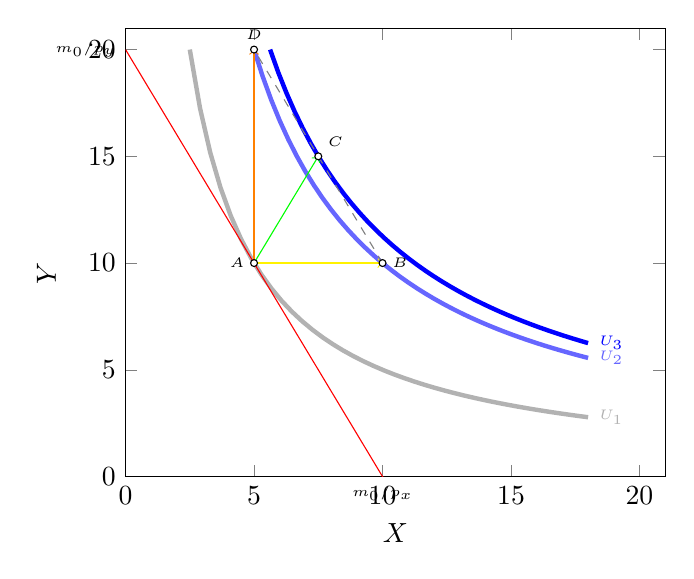
\begin{tikzpicture}
\tikzset{
every pin/.style={fill=yellow!50!white,rectangle,rounded corners=2pt,inner sep=2pt,font=\it\tiny},
small dot/.style={fill=black,circle,scale=0.3}
}
\begin{axis}[
	xmin=0,xmax=21,ymin=0,ymax=21,
	xlabel style={below},xlabel=$X$,
	ylabel style={left},ylabel=$Y$,
	extra x ticks={10},
	extra x tick style={tickwidth=0},
	extra x tick labels={{\tiny${m_0}/{p_x}$}},
	extra y ticks={20},
	extra y tick style={tickwidth=0},
	extra y tick labels={\tiny${m_0}/{p_y}$},
	samples=40]
\addplot[black!30,ultra thick,domain=2.5:18]
		{50/x} node[right] {\tiny $U_1$};
\addplot[blue!60,ultra thick,domain=5:18]
		{100/x} node[right] {\tiny $U_2$};
\addplot[blue,ultra thick,domain=5.625:18]
		{225/(2*x)} node[right] {\tiny $U_3$};
\addplot[red,domain=0:24]
		{20-2*x};							%涨价之后的预算线
\addplot[only marks,forget plot,black,mark options={mark size=1.25pt,fill=white},mark=*] coordinates {
	(10,10)
	(7.5,15)
	(5,10)
	(5,20)};
\node[left,font=\tiny]at (axis cs:5,10) {$A$};
\node[right,font=\tiny] at (axis cs:10,10) {$B$};
\node[above right,font=\tiny] at (axis cs:7.5,15) {$C$};
\node[above,font=\tiny] at (axis cs:5,20) {$D$};
\coordinate (equilibrium a) at (axis cs:5,10);
\coordinate (equilibrium b) at (axis cs:10,10);
\coordinate (equilibrium c) at (axis cs:7.5,15);
\coordinate (equilibrium d) at (axis cs:5,20);
\draw[yellow,->] (equilibrium a) -- (equilibrium b);
\draw[orange,->] (equilibrium a) -- (equilibrium d);
\draw[green,->] (equilibrium a) -- (equilibrium c);
\draw[gray,dashed] (equilibrium b) -- (equilibrium d);
\end{axis}
\end{tikzpicture}
\caption{\mbox{}}
\label{fig:cash-versus-goods-b}
\end{subfigure}
\caption{实物礼品和货币礼金}
\label{fig:cash-versus-goods}%
}}
\end{figure}

如图(\ref{fig:cash-versus-goods-a})所示,$X$是要送朋友的实物,$Y$是所有其他实物的复合品。要么赠送$\Delta x$数量的实物礼品,要么赠送与该实物礼品等价值的现金$\Delta m = \Delta x p_x$那么:
\begin{compactitem}
\item 在价格水平$(p_x, p_y)$和朋友的既定收入$m_0$下,原有的消费者均衡位于$A$点;
\item 送朋友$\Delta x$数量的$X$实物之后商品束由$A$点向右平移至$B$点,$\left | AB \right | = \Delta x$;
\item 假如当初送朋友$\Delta m$元现金,则等同于增加朋友的预算,在价格水平不变的前提下预算线外扩直至经过$B$点(与$B$的购买力一样);
\item 在新的预算约束$\Delta m + m_0$下,朋友达成新的消费者均衡$C$。
\end{compactitem}
注意,这个图示与分析只是一般意义上的讨论,其前提是朋友对所赠礼品和其他复合品的偏好满足严格凸性假设,属于良性偏好。至于完全偏好等类型大家可以自己画图分析。

或者如图(\ref{fig:cash-versus-goods-b}),根据良性偏好“平均束优于端点束”的假设进行分析,参看第\pageref{sec:well-behaved-preference}页。


\section*{推荐阅读}
\markright{推荐阅读}
\addcontentsline{toc}{section}{\hspace{-2.5em}推荐阅读}



\newpage
\section*{本章附录}
\markright{本章附录}
\addcontentsline{toc}{section}{\hspace{-2.5em}本章附录}
\label{sec:appendix-preferences-and-indifferent-curves}

\subsection*{凸集}


\subsection*{二元函数与曲面}